\documentclass[a4paper, 12pt,oneside]{book} % Here you chose the paper size and font size. The command onside ensures that pages are not shifted left and right (as is common for printed books). 
\usepackage[utf8]{inputenc} % Added to manage special characters, like Norwegian letters
\usepackage[T1]{fontenc} % To manage special characters
\usepackage{titlesec} % Used to change format for chapter titles
\titleformat{\chapter}[display]
  {\bfseries\Huge}  {\filright{\Large\chaptertitlename} \Huge\thechapter}
  {1ex}
  {}%}\vspace{1ex}\filleft}
  [\vspace{1ex}\titlerule]
%\usepackage[Bjarne]{fncychap} %fancy chapter style (many more available, like Sonny or Lenny etc.)
\usepackage{fancyhdr} %to customize the headers
\fancyhead{\nouppercase}
%\usepackage[lmargin=1in, rmargin=1in, tmargin=1.5in, bmargin=1.3in]{geometry} %sets the margins for the pages
\setcounter{tocdepth}{2} %table of contents number depth for subsections (2 = x.x.x)
\setcounter{secnumdepth}{4} %numbering depth for headers for subsections in the text(4 = x.x.x.x)
\usepackage{url} %to include urls
\usepackage{listings} %include this if you want to include code in the thesis
\usepackage{amsmath,amssymb} %mathematical package
\usepackage[per-mode=symbol]{siunitx} %includes SI-units
\usepackage[bf]{caption} %makes float captions bold
\usepackage{array, booktabs} %to make better tables
\usepackage{graphicx} %to include graphics
\usepackage{float} %to include floats
\usepackage[export]{adjustbox} %to adjust floats
\usepackage{subfig} %to include subfigures
\usepackage{chngcntr} %will make it possible to change the counter for tables, figures etc. such as below
\counterwithin{figure}{section} %change counter for figures within sections (also possible to choose for each chapter
\counterwithin{table}{section} %change counter for tables within sections
\usepackage{color, xcolor} %edit e.g. text colors
\usepackage{hyperref} %Adding internal links in you document
\hypersetup{
    colorlinks,
    citecolor=black,
    filecolor=black,
    linkcolor=black,
    urlcolor=black
}

% Here you can customize the look of your
% citations and bibliography
\usepackage[backend = biber,
            natbib = true, % Adding the natbib style
            % This will enable the use of \citet and \citep
            style = authoryear, % This can be changed to 
            % numerical if you only want numbers
            maxcitenames = 2,   % max number of 
            % names to include before et. al.
            ]{biblatex}
% Declare the bibliography resource
% (which you might want to connect to
% for example Zotero)
\addbibresource{bibliography.bib}
\usepackage{comment} %to be able to comment out sections in the .tex files
\usepackage{afterpage} %to customize page commands such as below
\usepackage[version=4]{mhchem} %Package for chemical notation
\newcommand\myemptypage{
    \null
    \thispagestyle{empty}
    \addtocounter{page}{-1}
    \newpage
    } %sets new page command to insert an empty page without adding to the page counter or having a page number




\begin{document}
%%%%%%%%%%%%%%%%%%%%%%%%%%%%%%%%%%%%%%%%%%%%%%%%%%%%%%%%
%\begin{comment}
% The title page:
% For NTNU students this page will be generated automatically when submitting your paper, and should not be included in the final file from Latex. Delete or comment out the title page setup. The final report should then start with the first page being the abstract. I have included a title page here so it is possible to see how it may look like, and for those who does not get an automatically generated title page. Of course you will need to change the names and titles etc. to your case.

%the title page should be an odd page (right hand side)

\begin{titlepage}
\vspace*{1.5cm}

\noindent  \textcolor{gray}{\large Ola Nordmann} \\
\vspace{1cm}

\noindent \textbf{\Large The title of your master's thesis should be written here} \\
\vspace{0.5cm}

\noindent {\large Any undertitle is written here} \\



\vspace{7cm}
\noindent Master's thesis in Geosciences \\
Supervisor: Supervisor Name \\
Co-supervisor: Co-supervisor Name \\
June 2025 \\

\vspace{0.2cm}
\noindent Norwegian University of Science and Technology \\
Faculty of Engineering \\
Department of Geoscience \\

\begin{figure}[h]
    
\includegraphics[width=0.28\textwidth]{Figures/ntnu_basic.png}
\end{figure}
\end{titlepage}


{%
  \sffamily
    \vbox{}\vfill
    {%
      \raggedleft
%     This template can be found at \\
%     \url{https://???} \\
%      \vspace{2cm}
      This template is an updated \\ 
      and expanded version of an \\
      earlier template created by \\
      Nina Salvesen. \\
    }%
    \vbox{}
}%

% The pre-chapters
\chapter*{Abstract} %pre-chapters should not be numbered, hExploratoryence the "*"
\pagenumbering{roman} %introductory pages should be roman
\setcounter{page}{1}
\addcontentsline{toc}{chapter}{\protect\numberline{}Abstract} %add the chapter to the table of contents, this is not automatically added when creating unnumbered chapters (*). Add it in a chapter style, and keep all chapters on the same numberline indent regardless of number or not on the chapter
This is a combined template and guideline for writing your project. This template should give the structure and a couple of examples, and it should help you get started on the different chapters of your thesis. You can clone and use this document template (\LaTeX) for your report. You do not need to follow all the guidelines given here, use your own judgment. The idea behind this document is rather to give you a reference for how to set up your document, and what is common to include in the different parts. What follows in this abstract can serve as an example of what will be presented in the other parts too. More information on how to write \LaTeX is given in Chap.~\ref{chap:Theory}, so please go directly to that chapter if you have not written in \LaTeX before.

The abstract is a short summary of your work. It should give the reader enough information to grasp the content of your work and decide whether they want to read it. When you read journal papers, you will see that they are usually just a single paragraph long. For a thesis, the abstract can be somewhat longer, but you should make an effort to try to keep it short and condensed. In general, an abstract should answer most of these questions:
\begin{itemize}
\item Why is the motivation for this work? Why is the study useful?
\item What is the research question? What has been studied?
\item What is(are) the objective(s)?
\item What methodology was used? (What has been done/how was it done?)
\item What are the main results?
\item What are the main conclusions?
\end{itemize}

 %insert the chapter text from the files

\chapter*{Preface}
\addcontentsline{toc}{chapter}{\protect\numberline{}Preface} 

Write the preface of your thesis here. \\

\noindent You may include acknowledgments and thanks as part of your preface on this page, or you may add it as a new chapter after the preface.

\tableofcontents
\addcontentsline{toc}{chapter}{\protect\numberline{}Contents}

%add to table of contents list of figures and tables, and insert list of figures and tables
\addcontentsline{toc}{chapter}{\protect\numberline{}\listfigurename}
\listoffigures
\addcontentsline{toc}{chapter}{\protect\numberline{}\listtablename}
\listoftables

\chapter*{Abbreviations}
\addcontentsline{toc}{chapter}{\protect\numberline{}Abbreviations}


% Put in your abbreviations here

List of all abbreviations in alphabetic order:

\begin{itemize}
    \item \textbf{IGV} Faculty for geosciences
    \item \textbf{NTNU} Norwegian University of Science and Technology
    \item \textbf{PCA} Principal Component Analysis
    
\end{itemize}
\newpage
\myemptypage
%add an empty non-counted page by the command below in order to get the first chapter on the left hand side, if needed (check your page number so that the first chapter is on an odd page)


%%%%%%%%%%%%%%%%%%%%%%%%%%%%%%%%%%%%%%%%%%%%%%%%%%%%%%%%
%Customize the layout of the main content of your thesis

%\pagestyle{fancy} %set customized page style for header
%\fancyhf{} %clear header and footer fields
%\renewcommand{\headrulewidth}{0pt} %set to no rule
%\fancyhead[LE, RO]{\thepage} %set the page number at left for even, right for odd pages
%\fancyhead[RE, LO]{\leftmark} %set the chapter name at right for even, left for odd pages
%is is possible to design the header with the chapter as you wish, e.q. only the chapter or only the name, all lowercase instead etc.
%you could also design the footer if you wish, for example:
%\fancyfoot[LE, RO]{\thepage}
%\setlength{\headheight}{14.49998pt} %set the header height


%%%%%%%%%%%%%%%%%%%%%%%%%%%%%%%%%%%%%%%%%%%%%%%%%%%%%%%%
%main content 

\pagenumbering{arabic}

\chapter{Introduction}
\label{chap:Introduction}

In your introduction, it is common to start with a broad focus and then narrow in. You could narrow it even further in the background section. The introduction section should give the perspective and background for your upcoming research question. This is where you can take an expansive and holistic view, before focusing on your question.

\section{Motivation}

It is common to have a motivation section in your introduction (it does not need to be singled out as a separate section, though; your motivation could be just a part of your introduction). In this section, you should motivate your research question, which will come later. Why is your work interesting? Why is it important? Why is it necessary? What is the purpose and aim of this work? This motivation should lead to the research question being asked later.

In this section, you should also distinguish your work from earlier studies. In the introduction, you should give a very brief overview of the current state of the art in the research field, and a more throughout discussion on earlier literature should be provided in the background chapter (Chapter \ref{chap:Background}). In this section, try to briefly point out what has already been done, what the earlier research showed, what the limitations of earlier research were, and how your work will address these shortcomings.


\subsection{Research question}

The research question you are trying to answer through your thesis should be formulated in the introduction section. The purpose of the motivation should lead to a hypothesis, and the research questions should be formulated so that they can verify the hypothesis.

You can also formulate a set of objectives for your work to answer your research question.  It should be clear how these objectives together will answer your research question.

\section{Outline}

It is common to end the introduction with an outline of the thesis. Here, you could briefly present the different chapters and their content.
\chapter{Background}
\label{chap:Background}

The background section should give sufficient background information to give the reader an overview of the state-of-the-art research field in which you work.

The background chapter can be a bit similar to the introduction. For journal articles, it is not that common with a background section, as it is not kept separate from the introduction. However, for a master thesis, it is common to have more background and therefore to separate out some of the background material into a separate chapter. For a specialization project, the background chapter could be the most important chapter, as the specialization project is centered around learning a new subject field.

Do not overestimate the background knowledge of the reader. As a rule of thumb, you could assume (s)he knows as much as you did when you started on your master thesis/project. So you need to give the reader enough background to be able to read the rest of your thesis.

All relevant literature should be included, so do a thorough literature search. When you do, try not to miss out on the classics and defining papers in your field of work. For a specialization project, your background section can include references to display the breadth of the field you are working on. In contrast, for a master thesis, you should be able to argue for all included references. Do not add references just to get a long reference list. After you have spent a lot of time reading something, it could be tempting to add those references to just show off that you have read them, even though it turned out after reading them that it is not fully related to your work. Do not, all included references in your master thesis should be relevant to your work.

The background material should also motivate your work. It should make your research question interesting by showing what others have done, and showing what is missing, highlighting the void that you try to fill with your work.


\section{Citations}

The background needs relevant literature to place your project work into context. The Google-scholar search (\url{scholar.google.com}) is a good starting point for searching for relevant papers.  This subsection will show how to include these references in your \LaTeX-document.

There is a long range of different styles and packages in Latex for citations. During your writing process, it is often beneficial to have an \texttt{authoryear} style, where you see the author(s) and the year of publication. This will help you remember what the reference is. In the \texttt{main.tex} file you will find a command defining the bibliography style:
\lstinputlisting[firstline=39, lastline=52]{main.tex}

This is where you want to go to change the style of your referencing. In this setup, we use the \texttt{natbib} style. This allows for using \verb=\citep= and \verb=\citet= references, which are useful if you use \texttt{authoryear} style:
\begin{itemize}
    \item Whenever the reference is part of the sentence, you should use the textual citation \verb=\citet=. The \verb=\citet= reference types will give a reference that looks like this: \citet{berg2014permeability}.
    \item Whenever the reference is not a part of the sentence, but just general for the sentence or paragraph, you should use the parenthetical citation \verb=\citep=. The \verb=\citep= reference types will give a reference that looks like this: \citep{berg2014permeability}.
    \item If you do not specify, but use \verb=\cite=, it will look like this: \cite{berg2014permeability}.
\end{itemize}

All the references you use will automatically show up in your reference list. If you want to shift to numerical citations, you should use the \texttt{cite} command, as there are no differences between textual and parenthetical citations when you use the numerical style.
\chapter{Theory}
\label{chap:Theory}

The theory section is not as common to include as the other sections included in this document. Some work is theory-heavy, and it can be beneficial to split the theory part from the background and methodology parts of the document. In this document, we will rather use this section to show some important \LaTeX commands that you are likely to use.

When you write in \LaTeX, try to just follow the given style. You might not like the exact way of the given style in your document, but if you try to change it with small commands everywhere, you will probably end up with a document that looks worse, and you will spend a lot of time writing \LaTeX code in your document.

\section{Equations}

A simple equation or variable can be written within sentences using the dollar sign on each side, for example, writing \verb=$a$= will show up as $a$. The usual way of including an equation on a separate line is either by using double dollar signs, such as this:
$$E = mc^2$$
or using the \texttt{equation} environment:
\begin{equation}
    E=mc^2
    \label{eq:Einstein}
\end{equation}
\sloppy Note that the \texttt{equation} environment will enumerate the equation, and allow you to add a label that you can refer to later. When labeling the equations, you can refer to them using \verb=\eqref{<label>}=, which will give you an equation reference like Eq.~\eqref{eq:Einstein}.

The text below shows an example of how to align equations on the equal sign, with only one reference for both. This may be useful for when they are linked and are actually only one equation but splitting them up makes it more readable.
\begin{equation}
\begin{aligned}
        a &= \sin^{2}(\Delta\phi/2) + a \sin^{2}(\Delta\phi/2) \\
         &= (1+a) \sin^{2}(\Delta\phi/2)
\end{aligned}
\label{eq:splitTwoLines}
\end{equation}
The whole equation can be referenced as a single equation, Eq.~\eqref{eq:splitTwoLines}. One may also align sub-equations such that they are numbered the same but have a letter differentiating them as shown below\footnote{A footnote explaining something.}. This can be used when they are linked, but you will need to reference both individual parts.

\begin{subequations}
\begin{align}
    \sigma &= \sqrt{\frac{1}{N} \sum_{i=1}^N (x_i - \mu)^2}
    \label{eq:sd}\\ 
    \mu &= \frac{1}{N} \sum_{i=1}^N x_i \label{eq:mean}
\end{align}
\label{eqn:subeqn}
\end{subequations}\\
These equations can be referenced by their specific sub-equation as Eq.~\eqref{eq:sd}, or by the whole group as Eqs.~\eqref{eqn:subeqn}.


\section{Including figures}

Figure \ref{fig:qualityDiff} is an example of how to include figures in your \LaTeX document. This is also an example of the difference between a vector-based image format (pdf) and a voxel-based format (png). When possible, always try to use a vector-based image format, as that gives infinite resolution.

These two figures were created using this simple Python code:

\lstinputlisting[firstline=1, lastline=17,language=Python]{Figures/createPlot.py}

So when you create figures using Python, try to save them as pdf, as use the tight boundaries to save some space around the figures.

\begin{figure}[H]
  \centering
  \subfloat[Sinus figure using pdf.]{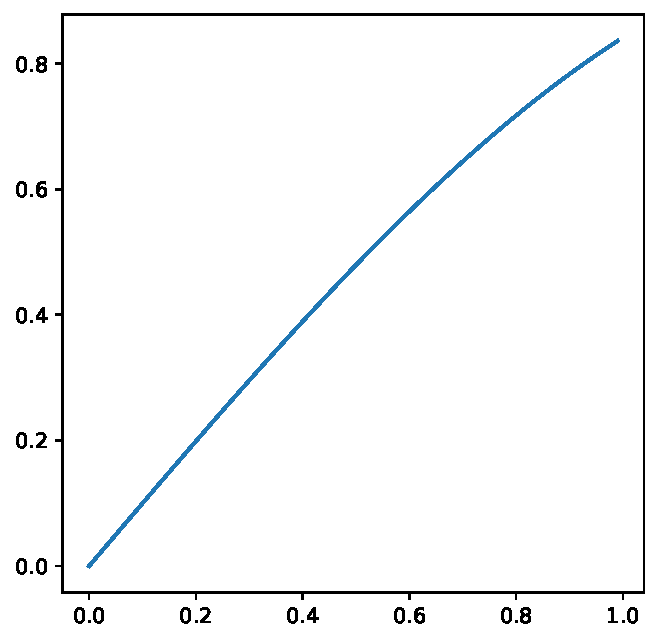
\includegraphics[width=0.45\textwidth]{Figures/sin.pdf}\label{fig:sinpdf}}
  \quad
  \subfloat[Sinus figures using png.]{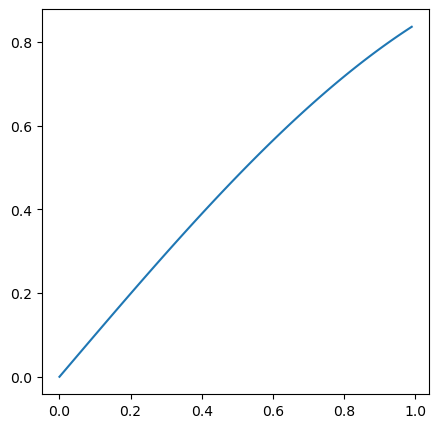
\includegraphics[width=0.45\textwidth]{Figures/sin.png}\label{fig:sinpng}}
  \caption{Figure (a) shows a pdf figure, while figure (b) shows a png figure. If you zoom in, you will start noticing the difference in quality.}
\label{fig:qualityDiff}
\end{figure}

With Python you could change the size of your figures. This is helpful for getting the right size of text within figures. In Figure \ref{fig:SizeDiff} we compare two different sizes.

\begin{figure}[H]
  \centering
  \subfloat[Sinus figure using size (8,8).]{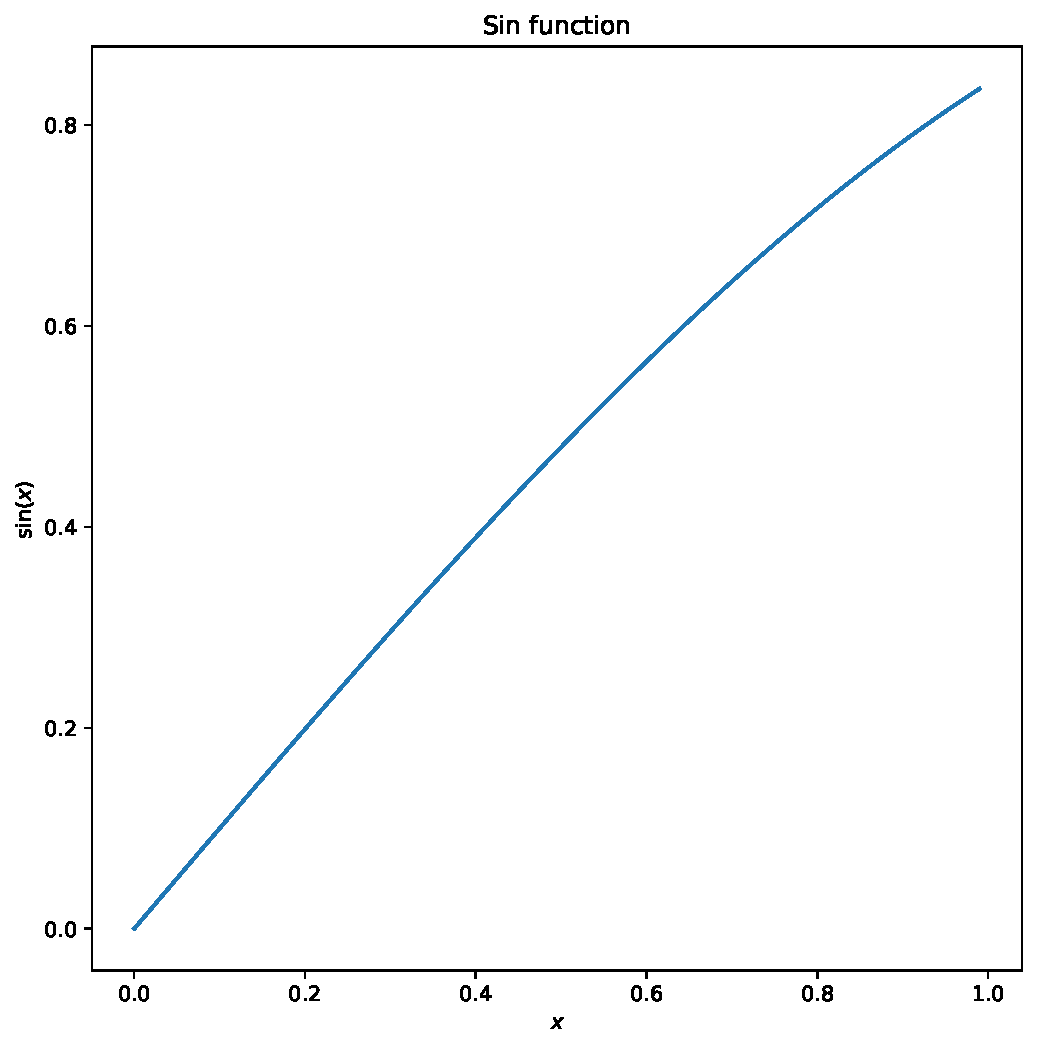
\includegraphics[width=0.45\textwidth]{Figures/sinBig.pdf}\label{fig:sinBig}}
  \quad
  \subfloat[Sinus figures using size (4,4).]{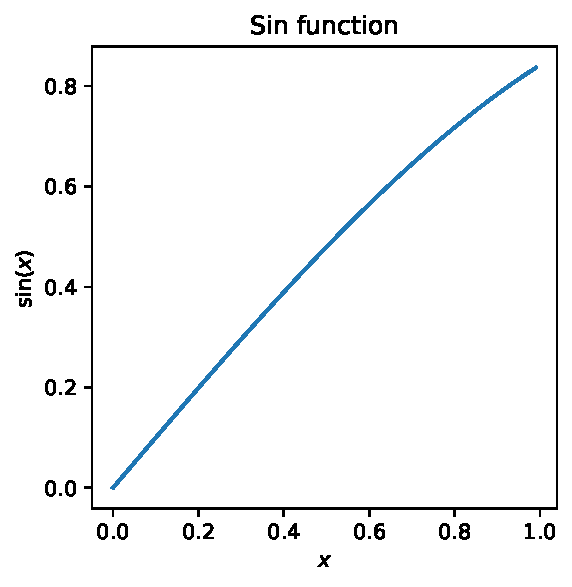
\includegraphics[width=0.45\textwidth]{Figures/sinSmall.pdf}\label{fig:sinSmall}}
  \caption{This is a comparison between two different figure sizes.}
\label{fig:SizeDiff}
\end{figure}


\section{Chemical notations and units}

This document has included a package for chemical symbols, \texttt{mchem}. When you write \verb=\ce{CO2}= you will get the chemical notation as \ce{CO2}.

For units we use the \texttt{siunitx} package. If you write \verb=\SI{10}{\meter\per\second\squared}= you get \SI{10}{\meter\per\second\squared}. The package can be used within math mode (inside the dollar signs). It automatically changes to a fixed notation for numbers, such as \verb=\SI{1E5}{\meter}= gives \SI{1E5}{\meter}.

\section{Tables}

Here are two examples of regular tables with data and a table with split headers.

\begin{table}[ht!]
\centering
    \begin{tabular}{ m{3cm} m{2.5cm} m{2.5cm} m{2.5cm} m{2cm} } 
    \toprule
    \toprule
    \textbf{Statistic} & \textbf{Velocity} & \textbf{Altitude} & \textbf{1/Angle} & \textbf{Temp.} \\
    \midrule
    Mean    & 122.68    & 240.98   & 93.75     & 13.95 \\[1.3ex]
    Std     & 224.51    & 145.88   & 60.39     & 4.44  \\[1.3ex]
    Q1      & 28.00     & 111.60   & 34.15     & 10.60 \\[1.3ex]
    Median  & 63.00     & 223.20   & 99.59     & 13.30 \\[1.3ex]
    Q3      & 137.00    & 359.10   & 151.99    & 16.70 \\[1.3ex]
    Min     & 0.00      & 1.00     & 0.00      & 3.30  \\[1.3ex]
    Max     & 14519.00  & 616.70   & 180.00    & 32.10 \\[1.3ex]
    \bottomrule
    \bottomrule
    \end{tabular}
% the square brackets after \caption gives the table a proper title in the list of tables, instead of just inserting the beginning of the table caption
\caption[Dynamic feature statistics with outliers]{Table of dynamic feature statistics where outliers are included, for all data points. Velocity is given in \textit{m/h}, the altitude in \textit{mamsl}, the inverse trajectory angle in 1/degrees, and temperature in degrees Celsius.}
\label{table:stat_fliers}
\end{table}


\begin{table}[ht!]
\centering
    \begin{tabular}{ m{3cm} m{5cm} m{3cm} } 
    \toprule
    \toprule
    \textbf{Area 1} & \textbf{Start date} & \textbf{End date} \\
    \midrule
    2018    & 03.06    & 29.06                       \\[1.3ex]
    2019    & 03.06    & 03.07 or 31.08\footnotemark \\[1.3ex]
    2020    & 03.06    & 05.09                       \\[1.3ex]
    \midrule
    \textbf{Area 2} & \textbf{Start date (farm 1/2)} & \textbf{End date} \\
    \midrule
    2012    & 09.06            & 07.09               \\[1.3ex]
    2013    & 23.06 / 15.06    & 25.08               \\[1.3ex]
    2014    & 05.06 / 25.06    & 10.09               \\[1.3ex]
    2015    & 13.06 / 03.07    & 06.09               \\[1.3ex]
    2016    & 17.06            & 22.07               \\[1.3ex]
    \bottomrule
    \bottomrule
    \end{tabular}
\caption[Selected time ranges for all data]{Selected time ranges for the data in all areas and all years.}
\label{table:time_ranges}
\end{table}

There are online tools to create \LaTeX tables. This might be a faster way of creating them than writing all the code yourself.

\chapter{Methods}

In this chapter, you describe the methods used to obtain your results. This can be new methods for analyzing existing data, or existing methods applied to new data. Include a complete description of your methods. It is often helpful to use flow charts to explain your methods.

Give enough details for others to be able to reproduce your work. Please do not overdo it, as a rule of thumb, you can assume that the reader has the same background as you had when you started the thesis.

Introduce and describe all parameters that have been tested in your project, and why these in particular have been varied. What was the reason for varying these parameters?

Additional details can be given in the appendices. Appendices are useful to avoid too much information in the thesis itself, which can be detrimental to the reading experience.

If you are developing or using software, then it is common to include pseudo-code for the software. The full code can be added as an appendix, but it is even better to upload the code to a public repository (e.g., \url{github.com}), and link the repository from the appendix.

\section{Writing tips}

Here are some general writing tips for best practices in scientific writing.

\begin{itemize}
    \item Use short sentences. Shorter sentences are easier for a reader to follow than longer sentences. As a rule of thumb, if you can split a sentence in two, it is usually for the better.
    \item Try to avoid adverbs and adjectives, e.g., quickly, slowly, densely, etc., as they are often not quantitative. A densely populated area in Finmark is not the same as a densely populated area in China.
    \begin{itemize}
        \item Avoid: The reaction completed quickly.
        \item Use: The reaction completed in 5 minutes.
    \end{itemize}
    \item If no one did the action, then it is sometimes common to avoid the passive voice. The active voice is usually clearer and more concise than the passive.
    \begin{itemize}
        \item Passive voice: Experiments were run.
        \item Active voice: We ran experiments.
    \end{itemize}
    \item Minimize the use of new abbreviations. As a reader, it is difficult to remember the meaning of more than a handful of new abbreviations. Commonly used symbols, such as $\phi$ for porosity, are an exception. If you do introduce numerous new abbreviations, it is useful to add a list of abbreviations at the beginning of your document (an example is included at the beginning of this document).
    \item A noun should follow \emph{this}, \emph{these}, etc.
    \begin{itemize}
        \item Avoid: This shows \dots
        \item Use: This result shows \dots
    \end{itemize}
    \item Avoid using \emph{it}, instead, try to be specific.
    \begin{itemize}
        \item Avoid: It revealed the importance of science.
        \item Use: The experiment revealed the importance of science.
    \end{itemize}
    \item Avoid "to be" verbs. Sentences with these verbs can almost always be shortened.
    \begin{itemize}
        \item Avoid: The reaction rate was decreasing.
        \item Use: The reaction rate decreased.
    \end{itemize}
    \item Be careful about verb tenses. Did something actually happen in the past, or are you presenting a result or observation that is still true today? Papers with numerical models are often written in the present tense, while papers focusing on experiments are often written in the past tense. But even in experimental papers, some sentences can be in the present tense if they refer to things that are still true, i.e., "The data shows \dots"
    \item Avoid putting words in quotations. If the idea or object needs quotations around something that describes it, then this usually means that you can find a better way to describe it.
    \begin{itemize}
        \item Avoid: The experiment modeled "serpentinization".
        \item Use: The experiment captured key aspects of the serpentinization process. 
    \end{itemize}
    \item Comma rules; \emph{that} does not follow a comma, whereas \emph{which} should follow a comma.
    \begin{itemize}
        \item Incorrect: The data, that we collected \dots
        \item Correct: The data that we collected \dots
        \item Incorrect: The students were angry which fueled the protests.
        \item Correct: The students were angry, which fueled the protests.
    \end{itemize}
    \item Contractions are common in speech and informal writing, but it is not used in formal writing.
    \begin{itemize}
        \item Use \emph{it is}, not \emph{it's}.
        \item Use \emph{does not}, not \emph{doesn't}.
        \item Use \emph{is not}, not \emph{isn't}.
        \item Use \emph{we will}, not \emph{we'll}.
    \end{itemize} 
    \item Some words are synonymous with others, but less common in formal scientific writing.
    \begin{itemize}
        \item Use \emph{although} instead of \emph{though}.
        \item Use \emph{in addition} or \emph{moreover} instead of \emph{besides}.
        \item Use \emph{however} instead of \emph{but}.
    \end{itemize}
\end{itemize}
\chapter{Results}
\label{chap:Results}

In this chapter, you describe the output from applying your methodology. Present your results in a clear manner, using a combination of figures and tables.

If you are doing lab experiments: What do you observe? Also include qualitative observations that might not be directly relevant (“We saw more production at the upper half of the core sample than the lower half, with most production leaving at the upper side-plane.”).

If you are doing computations: What is the output from applying your code/software? Which part of your software is using the most computational power? How does it compare to other similar software?

Illustrate the results. Use graphs, images, and tables (see Chapter \ref{chap:Theory}).

A common challenge is to distinguish the results and the discussion section. Do not discuss your results in this chapter, that should be done in the discussion section. If it is hard to separate results and discussion, you might combine them into one section. You could also split the results and discussion part of your thesis into several results/discussion sections for different topics (“Magnesium effect on imbibition”, “Sodium effect on imbibition”).

Try to avoid repetition between. In case you have many graphs of the same process, keep some characteristic graphs and move the rest to an appendix. Then you describe one graph in detail and refer to the others in the appendix for changes between the results.
\chapter{Discussion}

In this chapter, you should expand on your results and address your main research questions (the research questions were stated in Chapter \ref{chap:Introduction}). You should post-process and discuss the results already presented in Chapter \ref{chap:Results}.

What kind of information can you deduce based on the results you have compiled and presented in the Result section? How do the different results you have obtained compare to what you expected or to results reported by others? Cross-plot your results to extract information. Discuss variation between re-runs.

What do the results tell us? Try to answer your research questions. Provide the information you said you wanted to provide by conducting this study. Can you draw conclusions, and in particular, can you answer your research question? Can you give a negative answer? If not, is a positive answer probable?
\chapter{Conclusions}

Give a concise summary of your research and findings here, and include a short summary of any future work as well.

You could also discuss the consequences and possible applications of your results. What does your result have to say for your scientific field? What are the economic consequences if your results are commercialized? What are the consequences for the society and environment?

\section{Future work}

Include a section about what should or could be done in future research, or explain any recommended next steps based on the results you got. This should be the last section of the conclusion chapter.

\addcontentsline{toc}{chapter}{\protect\numberline{}References}
\printbibliography[title={References}] %you may change the title in the toc here if you want
\cleardoublepage

\chapter*{\LARGE \textbf{Appendices}}
\fancyhf{} %clear the header, it should be empty for the appendices
\renewcommand{\headrulewidth}{0pt} %no rule
\fancyfoot[C]{\thepage} %set the page numbers in the center of the footer instead 

%it is possible to set a different page numbering style for the appendix, but I personally just continued with the same page numbering as the main content as I find that more tidy
%\pagenumbering{roman}
%\setcounter{page}{1}
\addcontentsline{toc}{chapter}{\protect\numberline{}Appendices:}
\appendix


\chapter*{A - Github repository}
\addcontentsline{toc}{chapter}{\protect\numberline{}A - Github repository} 

Codes and input files can be uploaded to a repository. Below is a link to a GitHub repository for a specialization project:


\subsection*{Github repository link}
\begin{itemize}
    \item \url{https://github.com/Adelved/specialization-project}
\end{itemize}


%%%%%%%%%%%%%%%%%%%%%%%%%%%%%%%%%%%%%%%%%%%%%%%%%%%%%%%%



\end{document}
